\documentclass[a4paper]{book}
\usepackage{a4wide}
\usepackage{makeidx}
\usepackage{fancyhdr}
\usepackage{graphicx}
\usepackage{multicol}
\usepackage{float}
\usepackage{textcomp}
\usepackage{alltt}
\usepackage{times}
\usepackage{ifpdf}
\ifpdf
\usepackage[pdftex,
            pagebackref=true,
            colorlinks=true,
            linkcolor=blue,
            unicode
           ]{hyperref}
\else
\usepackage[ps2pdf,
            pagebackref=true,
            colorlinks=true,
            linkcolor=blue,
            unicode
           ]{hyperref}
\usepackage{pspicture}
\fi
\usepackage[utf8]{inputenc}
\usepackage{doxygen}
\makeindex
\setcounter{tocdepth}{3}
\renewcommand{\footrulewidth}{0.4pt}
\begin{document}
\begin{titlepage}
\vspace*{7cm}
\begin{center}
{\Large Nessie, reconocedor óptico de texto en recortes de prensa escrita \\[1ex]\large 1.0 }\\
\vspace*{1cm}
{\large Generated by Doxygen 1.5.6}\\
\vspace*{0.5cm}
{\small Thu Sep 18 11:25:12 2008}\\
\end{center}
\end{titlepage}
\clearemptydoublepage
\pagenumbering{roman}
\tableofcontents
\clearemptydoublepage
\pagenumbering{arabic}
\chapter{Directory Hierarchy}
\section{Directories}
This directory hierarchy is sorted roughly, but not completely, alphabetically:\begin{CompactList}
\item \contentsline{section}{inc}{\pageref{dir_ef15eccf5bd9eca446a41a18c57ac0fd}}{}
\item \contentsline{section}{src}{\pageref{dir_f108b8e716a38a781a23bf0e62a4b450}}{}
\end{CompactList}

\chapter{Data Structure Index}
\subsection{Data Structures}
Here are the data structures with brief descriptions:\begin{CompactList}
\item\contentsline{section}{\hyperlink{class_clip}{Clip} (Press clip where the recognizer has to extract the text from )}{\pageref{class_clip}}{}
\item\contentsline{section}{\hyperlink{class_clip_location}{ClipLocation} (Location of a press clip inside a newspaper page )}{\pageref{class_clip_location}}{}
\item\contentsline{section}{\hyperlink{class_nessie_exception}{NessieException} (Exception raised by a Nessie OCR object )}{\pageref{class_nessie_exception}}{}
\item\contentsline{section}{\hyperlink{class_preprocessor}{Preprocessor} (\hyperlink{class_preprocessor}{Preprocessor} of the OCR process )}{\pageref{class_preprocessor}}{}
\item\contentsline{section}{\hyperlink{class_recognizer}{Recognizer} (Manager of the whole OCR process )}{\pageref{class_recognizer}}{}
\item\contentsline{section}{\hyperlink{class_segmenter}{Segmenter} (\hyperlink{class_segmenter}{Segmenter} of the OCR process )}{\pageref{class_segmenter}}{}
\item\contentsline{section}{\hyperlink{class_shape}{Shape} (The shape of a character in a press clip )}{\pageref{class_shape}}{}
\item\contentsline{section}{\hyperlink{class_statistics}{Statistics} (Statistical data regarding the text recognition process )}{\pageref{class_statistics}}{}
\item\contentsline{section}{\hyperlink{class_text}{Text} (\hyperlink{class_text}{Text} extracted by the recognizer )}{\pageref{class_text}}{}
\end{CompactList}

\chapter{Directory Documentation}
\hypertarget{dir_ef15eccf5bd9eca446a41a18c57ac0fd}{
\section{inc/ Directory Reference}
\label{dir_ef15eccf5bd9eca446a41a18c57ac0fd}\index{inc/ Directory Reference@{inc/ Directory Reference}}
}




\nopagebreak
\begin{figure}[H]
\begin{center}
\leavevmode
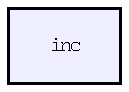
\includegraphics[width=49pt]{dir_ef15eccf5bd9eca446a41a18c57ac0fd_dep}
\end{center}
\end{figure}
\subsection*{Files}
\begin{CompactItemize}
\item 
file \textbf{Classifier.hpp}
\item 
file \hyperlink{_clip_8hpp}{Clip.hpp}
\begin{CompactList}\small\item\em Declaration of the class \hyperlink{class_clip}{Clip}. \item\end{CompactList}

\item 
file \hyperlink{_clip_location_8hpp}{ClipLocation.hpp}
\begin{CompactList}\small\item\em Declaration of the class \hyperlink{class_clip_location}{ClipLocation}. \item\end{CompactList}

\item 
file \textbf{FeatureVector.hpp}
\item 
file \hyperlink{_nessie_exception_8hpp}{NessieException.hpp}
\begin{CompactList}\small\item\em Declaration of the class \hyperlink{class_nessie_exception}{NessieException}. \item\end{CompactList}

\item 
file \hyperlink{_pixel_8hpp}{Pixel.hpp}
\begin{CompactList}\small\item\em Declaration of the custom type Pixel. \item\end{CompactList}

\item 
file \hyperlink{_preprocessor_8hpp}{Preprocessor.hpp}
\begin{CompactList}\small\item\em Declaration of the class \hyperlink{class_preprocessor}{Preprocessor}. \item\end{CompactList}

\item 
file \hyperlink{_recognizer_8hpp}{Recognizer.hpp}
\begin{CompactList}\small\item\em Declaration of the class \hyperlink{class_recognizer}{Recognizer}. \item\end{CompactList}

\item 
file \hyperlink{_segmenter_8hpp}{Segmenter.hpp}
\begin{CompactList}\small\item\em Declaration of the class \hyperlink{class_segmenter}{Segmenter}. \item\end{CompactList}

\item 
file \hyperlink{_shape_8hpp}{Shape.hpp}
\begin{CompactList}\small\item\em Declaration of the class \hyperlink{class_shape}{Shape}. \item\end{CompactList}

\item 
file \hyperlink{_statistics_8hpp}{Statistics.hpp}
\begin{CompactList}\small\item\em Declaration of the class \hyperlink{class_statistics}{Statistics}. \item\end{CompactList}

\item 
file \hyperlink{_text_8hpp}{Text.hpp}
\begin{CompactList}\small\item\em Declaration of the class \hyperlink{class_text}{Text}. \item\end{CompactList}

\end{CompactItemize}

\hypertarget{dir_f108b8e716a38a781a23bf0e62a4b450}{
\section{src/ Directory Reference}
\label{dir_f108b8e716a38a781a23bf0e62a4b450}\index{src/ Directory Reference@{src/ Directory Reference}}
}




\nopagebreak
\begin{figure}[H]
\begin{center}
\leavevmode
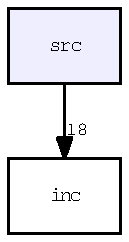
\includegraphics[width=49pt]{dir_f108b8e716a38a781a23bf0e62a4b450_dep}
\end{center}
\end{figure}
\subsection*{Files}
\begin{CompactItemize}
\item 
file \textbf{Classifier.cpp}
\item 
file \hyperlink{_clip_8cpp}{Clip.cpp}
\begin{CompactList}\small\item\em Implementation of the class \hyperlink{class_clip}{Clip}. \item\end{CompactList}

\item 
file \hyperlink{_clip_location_8cpp}{ClipLocation.cpp}
\begin{CompactList}\small\item\em Implementation of the class \hyperlink{class_clip_location}{ClipLocation}. \item\end{CompactList}

\item 
file \textbf{FeatureVector.cpp}
\item 
file \hyperlink{main_8cpp}{main.cpp}
\begin{CompactList}\small\item\em Implementation of a command line program for testing purposes. \item\end{CompactList}

\item 
file \hyperlink{_nessie_exception_8cpp}{NessieException.cpp}
\begin{CompactList}\small\item\em Implementation of the class \hyperlink{class_nessie_exception}{NessieException}. \item\end{CompactList}

\item 
file \hyperlink{_preprocessor_8cpp}{Preprocessor.cpp}
\begin{CompactList}\small\item\em Implementation of the class \hyperlink{class_preprocessor}{Preprocessor}. \item\end{CompactList}

\item 
file \hyperlink{_recognizer_8cpp}{Recognizer.cpp}
\begin{CompactList}\small\item\em Implementation of the class \hyperlink{class_recognizer}{Recognizer}. \item\end{CompactList}

\item 
file \hyperlink{_segmenter_8cpp}{Segmenter.cpp}
\begin{CompactList}\small\item\em Definition of the class \hyperlink{class_segmenter}{Segmenter}. \item\end{CompactList}

\item 
file \hyperlink{_shape_8cpp}{Shape.cpp}
\begin{CompactList}\small\item\em Implementation of the class \hyperlink{class_shape}{Shape}. \item\end{CompactList}

\item 
file \hyperlink{_statistics_8cpp}{Statistics.cpp}
\begin{CompactList}\small\item\em Implementation of the class \hyperlink{class_statistics}{Statistics}. \item\end{CompactList}

\item 
file \hyperlink{_text_8cpp}{Text.cpp}
\begin{CompactList}\small\item\em Implementation of the class \hyperlink{class_text}{Text}. \item\end{CompactList}

\end{CompactItemize}

\chapter{Data Structure Documentation}
\hypertarget{struct_statistics}{
\section{Statistics Struct Reference}
\label{struct_statistics}\index{Statistics@{Statistics}}
}
{\tt \#include $<$Statistics.h$>$}



\subsection{Detailed Description}
\hyperlink{struct_statistics}{Statistics} about a text and its recognition process. 

This struct stores a number of statistic data regarding the recognition process and the text produced.

First, it stores the elapsed time on every stage, accumulated internally in the critical processes (mostly, image processing algorithms). Second, it also stores the number of words in the text and the appearance rate of every single word.

\begin{Desc}
\item[Author:]Eliezer Talón (\href{mailto:elitalon@gmail.com}{\tt elitalon@gmail.com}) \end{Desc}
\begin{Desc}
\item[Date:]2008-09-18 \end{Desc}


Definition at line 24 of file Statistics.h.\subsection*{Public Member Functions}
\begin{CompactItemize}
\item 
\hyperlink{struct_statistics_60ddd90a571ed4c3ce8c0f6317a36d63}{Statistics} ()
\begin{CompactList}\small\item\em Constructor. \item\end{CompactList}\item 
\hyperlink{struct_statistics_b68ede75479e44d5c35b78ec1284065b}{$\sim$Statistics} ()
\begin{CompactList}\small\item\em Destructor. \item\end{CompactList}\end{CompactItemize}
\subsection*{Data Fields}
\begin{CompactItemize}
\item 
\hypertarget{struct_statistics_b8aec77e19e962544468c569a8333d15}{
unsigned int \hyperlink{struct_statistics_b8aec77e19e962544468c569a8333d15}{nWords}}
\label{struct_statistics_b8aec77e19e962544468c569a8333d15}

\begin{CompactList}\small\item\em Number of words in the recognized text. \item\end{CompactList}\item 
\hypertarget{struct_statistics_905896f578b6af9e46d82990e39480bd}{
vector$<$ \hyperlink{_word_rate_8h_e8f43926daba5798edbb3cb94ad07ff7}{WordRate} $>$ \hyperlink{struct_statistics_905896f578b6af9e46d82990e39480bd}{wordRates}}
\label{struct_statistics_905896f578b6af9e46d82990e39480bd}

\begin{CompactList}\small\item\em List of appearance rates of every word in the recognized text. \item\end{CompactList}\item 
\hypertarget{struct_statistics_4a194feb4de2fc619d311b2adb2a7e74}{
double \hyperlink{struct_statistics_4a194feb4de2fc619d311b2adb2a7e74}{noiseRemovalTime}}
\label{struct_statistics_4a194feb4de2fc619d311b2adb2a7e74}

\begin{CompactList}\small\item\em Elapsed time in the noise removal stage. \item\end{CompactList}\item 
\hypertarget{struct_statistics_fc22ca2705714cfc44c45c772475c1cb}{
double \hyperlink{struct_statistics_fc22ca2705714cfc44c45c772475c1cb}{grayscaleConversionTime}}
\label{struct_statistics_fc22ca2705714cfc44c45c772475c1cb}

\begin{CompactList}\small\item\em Elapsed time in the grayscale conversion stage. \item\end{CompactList}\item 
\hypertarget{struct_statistics_6c2cd48482d1de181cb2dd32b3315449}{
double \hyperlink{struct_statistics_6c2cd48482d1de181cb2dd32b3315449}{floodFillingTime}}
\label{struct_statistics_6c2cd48482d1de181cb2dd32b3315449}

\begin{CompactList}\small\item\em Elapsed time in the flood filling stage. \item\end{CompactList}\item 
\hypertarget{struct_statistics_e2c88c8b599b217ad3f316cca7a15a23}{
double \hyperlink{struct_statistics_e2c88c8b599b217ad3f316cca7a15a23}{thresholdingTime}}
\label{struct_statistics_e2c88c8b599b217ad3f316cca7a15a23}

\begin{CompactList}\small\item\em Elapsed time in the thresholding stage. \item\end{CompactList}\item 
\hypertarget{struct_statistics_ae46d5f7b2a374dd79b15533facc9e6c}{
double \hyperlink{struct_statistics_ae46d5f7b2a374dd79b15533facc9e6c}{featureVectorsBuildingTime}}
\label{struct_statistics_ae46d5f7b2a374dd79b15533facc9e6c}

\begin{CompactList}\small\item\em Elapsed time in the feature vectors building stage. \item\end{CompactList}\item 
\hypertarget{struct_statistics_1e09de36cf3a65ab2a471e877578257d}{
double \hyperlink{struct_statistics_1e09de36cf3a65ab2a471e877578257d}{charactersExtractionTime}}
\label{struct_statistics_1e09de36cf3a65ab2a471e877578257d}

\begin{CompactList}\small\item\em Elapsed time in the characters extraction stage. \item\end{CompactList}\item 
\hypertarget{struct_statistics_7bfcefbca86812a13371f35f6ad2632c}{
double \hyperlink{struct_statistics_7bfcefbca86812a13371f35f6ad2632c}{classificationTime}}
\label{struct_statistics_7bfcefbca86812a13371f35f6ad2632c}

\begin{CompactList}\small\item\em Returns the total time within the classification stage. \item\end{CompactList}\item 
\hypertarget{struct_statistics_f5afa8bf14678df2d5b869b6161a209f}{
double \hyperlink{struct_statistics_f5afa8bf14678df2d5b869b6161a209f}{segmentationTime}}
\label{struct_statistics_f5afa8bf14678df2d5b869b6161a209f}

\begin{CompactList}\small\item\em Returns the total time within the segmentation stage. \item\end{CompactList}\item 
\hypertarget{struct_statistics_57aa8970c666c415db6dcdd0cc3920f6}{
double \hyperlink{struct_statistics_57aa8970c666c415db6dcdd0cc3920f6}{preprocessingTime}}
\label{struct_statistics_57aa8970c666c415db6dcdd0cc3920f6}

\begin{CompactList}\small\item\em Returns the total time within the preprocessing stage. \item\end{CompactList}\end{CompactItemize}


\subsection{Constructor \& Destructor Documentation}
\hypertarget{struct_statistics_60ddd90a571ed4c3ce8c0f6317a36d63}{
\index{Statistics@{Statistics}!Statistics@{Statistics}}
\index{Statistics@{Statistics}!Statistics@{Statistics}}
\subsubsection[Statistics]{\setlength{\rightskip}{0pt plus 5cm}Statistics::Statistics ()}}
\label{struct_statistics_60ddd90a571ed4c3ce8c0f6317a36d63}


Constructor. 

Initializes a \hyperlink{struct_statistics}{Statistics} object with timers set to 0

\begin{Desc}
\item[Author:]Eliezer Talón (\href{mailto:elitalon@gmail.com}{\tt elitalon@gmail.com}) \end{Desc}
\begin{Desc}
\item[Date:]2008-09-22 \end{Desc}


Definition at line 10 of file Statistics.cpp.\hypertarget{struct_statistics_b68ede75479e44d5c35b78ec1284065b}{
\index{Statistics@{Statistics}!$\sim$Statistics@{$\sim$Statistics}}
\index{$\sim$Statistics@{$\sim$Statistics}!Statistics@{Statistics}}
\subsubsection[$\sim$Statistics]{\setlength{\rightskip}{0pt plus 5cm}Statistics::$\sim$Statistics ()}}
\label{struct_statistics_b68ede75479e44d5c35b78ec1284065b}


Destructor. 

Destroys a \hyperlink{struct_statistics}{Statistics} object

\begin{Desc}
\item[Author:]Eliezer Talón (\href{mailto:elitalon@gmail.com}{\tt elitalon@gmail.com}) \end{Desc}
\begin{Desc}
\item[Date:]2008-09-17 \end{Desc}


Definition at line 25 of file Statistics.cpp.

The documentation for this struct was generated from the following files:\begin{CompactItemize}
\item 
Statistics.h (111)\item 
Statistics.cpp (111)\end{CompactItemize}

\hypertarget{struct_word_rate}{
\section{WordRate Struct Reference}
\label{struct_word_rate}\index{WordRate@{WordRate}}
}
{\tt \#include $<$WordRate.h$>$}



\subsection{Detailed Description}
Appearance rate of a word. 

This structure keeps the number of appearances of a single word in the recognized text from an clip.

\begin{Desc}
\item[Author:]Eliezer Talón (\href{mailto:elitalon@gmail.com}{\tt elitalon@gmail.com}) \end{Desc}
\begin{Desc}
\item[Date:]2008-09-18 \end{Desc}


Definition at line 17 of file WordRate.h.\subsection*{Public Member Functions}
\begin{CompactItemize}
\item 
\hyperlink{struct_word_rate_c22aaa0c04769cce44ba08bf5e6eb655}{WordRate} ()
\begin{CompactList}\small\item\em Constructor. \item\end{CompactList}\item 
\hyperlink{struct_word_rate_a86a63516e4c3d4e8aa9060ea5be6b23}{$\sim$WordRate} ()
\begin{CompactList}\small\item\em Destructor. \item\end{CompactList}\end{CompactItemize}
\subsection*{Data Fields}
\begin{CompactItemize}
\item 
\hypertarget{struct_word_rate_38d2adc9d4f6463bd66916be8f52d5f4}{
string \hyperlink{struct_word_rate_38d2adc9d4f6463bd66916be8f52d5f4}{word}}
\label{struct_word_rate_38d2adc9d4f6463bd66916be8f52d5f4}

\begin{CompactList}\small\item\em The word itself. \item\end{CompactList}\item 
\hypertarget{struct_word_rate_7e72f43d0fd5042d844f2cb234d11568}{
unsigned int \hyperlink{struct_word_rate_7e72f43d0fd5042d844f2cb234d11568}{rate}}
\label{struct_word_rate_7e72f43d0fd5042d844f2cb234d11568}

\begin{CompactList}\small\item\em Number of appearances. \item\end{CompactList}\end{CompactItemize}


\subsection{Constructor \& Destructor Documentation}
\hypertarget{struct_word_rate_c22aaa0c04769cce44ba08bf5e6eb655}{
\index{WordRate@{WordRate}!WordRate@{WordRate}}
\index{WordRate@{WordRate}!WordRate@{WordRate}}
\subsubsection[WordRate]{\setlength{\rightskip}{0pt plus 5cm}WordRate::WordRate ()}}
\label{struct_word_rate_c22aaa0c04769cce44ba08bf5e6eb655}


Constructor. 

Initializes a \hyperlink{struct_word_rate}{WordRate} object with an empty string and 0 appearances.

\begin{Desc}
\item[Author:]Eliezer Talón (\href{mailto:elitalon@gmail.com}{\tt elitalon@gmail.com}) \end{Desc}
\begin{Desc}
\item[Date:]2008-09-18 \end{Desc}


Definition at line 10 of file WordRate.cpp.\hypertarget{struct_word_rate_a86a63516e4c3d4e8aa9060ea5be6b23}{
\index{WordRate@{WordRate}!$\sim$WordRate@{$\sim$WordRate}}
\index{$\sim$WordRate@{$\sim$WordRate}!WordRate@{WordRate}}
\subsubsection[$\sim$WordRate]{\setlength{\rightskip}{0pt plus 5cm}WordRate::$\sim$WordRate ()}}
\label{struct_word_rate_a86a63516e4c3d4e8aa9060ea5be6b23}


Destructor. 

Destroys a \hyperlink{struct_word_rate}{WordRate} object.

\begin{Desc}
\item[Author:]Eliezer Talón (\href{mailto:elitalon@gmail.com}{\tt elitalon@gmail.com}) \end{Desc}
\begin{Desc}
\item[Date:]2008-09-17 \end{Desc}


Definition at line 22 of file WordRate.cpp.

The documentation for this struct was generated from the following files:\begin{CompactItemize}
\item 
WordRate.h (109)\item 
WordRate.cpp (109)\end{CompactItemize}

\printindex
\end{document}
